In Fig. \ref{fig:3.8.2_motion_plane_motion_in_a_plane},  $\vec{A}$ denotes the velocity of the boat, $
\vec{B}$ denotes the water current and $\vec{C}$ represents the resultant velocity. 

 \begin{align}
\vec{A} &=\myvec{0\\25} \label{eq:constr_a_motion_in_a_plane}\\
\vec{B} &=10\myvec{\cos 30\degree\\ -\sin 30\degree} \label{eq:constr_b_motion_in_a_plane}\\
\vec{C} &= \vec{A} + \vec{B}\\
&=5\myvec{\sqrt{3} \\4}
\end{align}
The following Python code generates Fig. \ref{fig:3.8.2_motion_plane_motion_in_a_plane}

\begin{lstlisting}
solutions/2/codes/line_ex/motion_in_a_plane/motion_plane.py
\end{lstlisting}

 \begin{figure}[!ht]
\centering
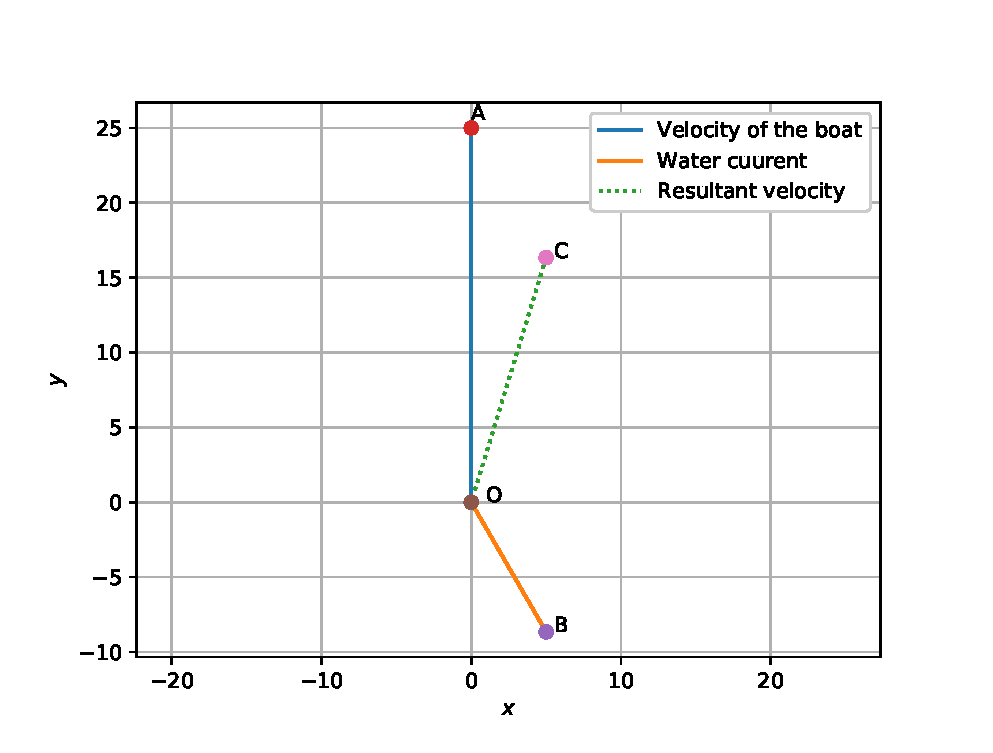
\includegraphics[width=\columnwidth]{./solutions/2/figs/line_ex/motion_in_a_plane/motion_plane.eps}
\caption{}
\label{fig:3.8.2_motion_plane_motion_in_a_plane}
\end{figure} 


